\chapter{Diseño}
\vspace*{-0.65cm}
En este capítulo se presenta el diseño completo del sistema de monitorización desarrollado. Tras la definición de los requisitos funcionales y no funcionales y la metodología de trabajo, se describe la arquitectura general y la estructura de red utilizada como base para la implementación.
\vspace*{-0.75cm}
\section{Arquitectura general del sistema}

El sistema se ha concebido bajo una arquitectura de tipo cliente-servidor organizada en tres capas diferenciadas: la capa de presentación (frontend), la capa lógica y de procesamiento (backend) y la capa de dispositivos de red monitorizados (routers Cisco). Esta estructura permite separar de manera clara las responsabilidades de cada componente, facilita la escalabilidad del sistema y permite una evolución modular de las funcionalidades.

La Figura~\ref{fig:arquitectura_general} muestra la arquitectura global del sistema y las relaciones entre sus componentes principales.

\begin{figure}[H]
\centering
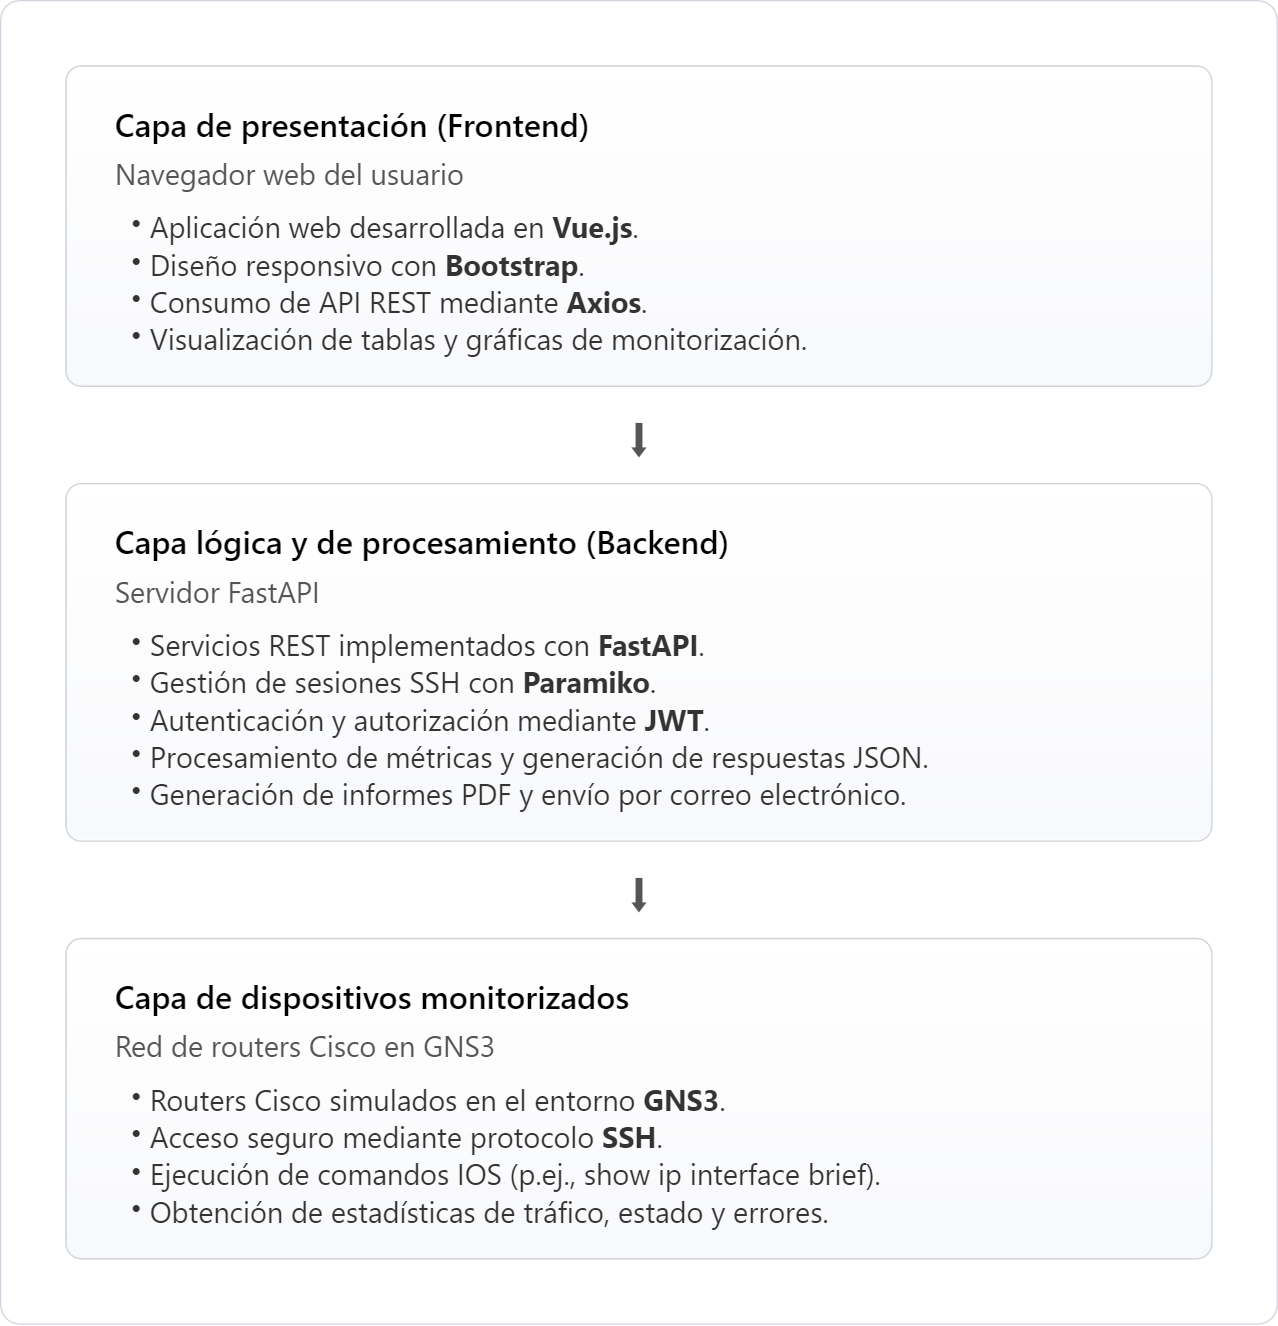
\includegraphics[width=0.7\textwidth]{canva/arquitectura_general.png}
\caption{Arquitectura general del sistema: interacción entre frontend, backend y routers Cisco.}
\label{fig:arquitectura_general}
\end{figure}

\subsection*{Capa de presentación (Frontend)}

La capa de presentación está implementada mediante una aplicación web desarrollada con Vue.js, Bootstrap y Axios. Su función principal es proporcionar una interfaz gráfica intuitiva que permita al usuario autenticado visualizar el estado de los routers, consultar estadísticas de tráfico, identificar errores, gestionar interfaces y visualizar informes generados automáticamente. El frontend interactúa exclusivamente con el backend a través de peticiones HTTP basadas en el estilo arquitectónico REST, sin acceder directamente a los routers. Esta separación facilita la centralización de la lógica de negocio y simplifica la seguridad del sistema.

\begin{itemize}
    \item Autenticación de usuarios: basada en JSON Web Tokens (JWT), garantizando que únicamente usuarios autorizados puedan acceder a los datos de monitorización.
    \item Conexión SSH con los routers: mediante la librería Paramiko, el backend establece sesiones seguras con los routers Cisco para la ejecución de comandos IOS en tiempo real.
    \item Procesamiento de datos: tras la ejecución de los comandos, el servidor interpreta y estructura la salida del router en formato JSON, de modo que pueda ser consumida de forma eficiente por el frontend.
    \item Gestión de alertas e informes: el backend detecta errores nuevos en las interfaces, genera informes en formato PDF y los remite por correo electrónico al usuario autenticado.
    \item Persistencia de datos: mediante una base de datos relacional que almacena usuarios, routers configurados, errores detectados y registros históricos.
\end{itemize}

En esta capa se produce toda la interacción con los dispositivos de red, garantizando seguridad, control y tratamiento homogéneo de la infromación recibida.

\subsection*{Capa de dispositivos monitorizados (Routers Cisco).}

La tercera capa está formada por los routers Csico simulados en el entorno de GNS3. Estos dispositivos consituyen la fuente de información del sistema, pues exponen sus estadísticas y estado operativo a través de sesiones SSH.

Los routers ejecutan comandos IOS tales como \texttt{show ip interface brief}, \texttt{show interfaces} o \texttt{show processes cpu}, que son utilizados por el backend para elaborar los resumenes de estado, gráficas de tráfico o detección de errores.

La comunicación se establece mediante el protocolo SSH, que garantiza autenticación, integridad y confidencialidad en el intercambio de datos. Al emplear este protocolo, el sistema puede monitorizar dispositivos reales o simulados sin exponer información sensible en texto plano.

\section{Diseño de la red en GNS3}

Para validar el funcionamiento del sistema de monitorización desarrollado se diseñó una red de pruebas en el simulador GNS. Esta red constituye un entorno controlado que reproduce de manera realista el comportamientop de una interfaz Cisco, permitiendo ejecutar comandos IOS, monitorizar interfaces, forzar errores y capturar métricas en tiempo real. En esta sección se describen la topología empleada, los dispositivos que la conforman y el dereccionamiento utilizado.

\subsection*{Topología general}

La topología final, mostrada en la Figura~\ref{fig:topologia_gns3}, está compuesta por tres routers Cisco (R1, R2 y R3), un switch de distribución y un nodo \textit{Cloud} que proporciona conectividad directa con la máquina virtual UbuntuGNS3, utilizada como servidor del sistema. Esta estructura permite simular tanto enlaces punto a punto como una red local común a los tres routers.

\begin{figure}[H]
\centering
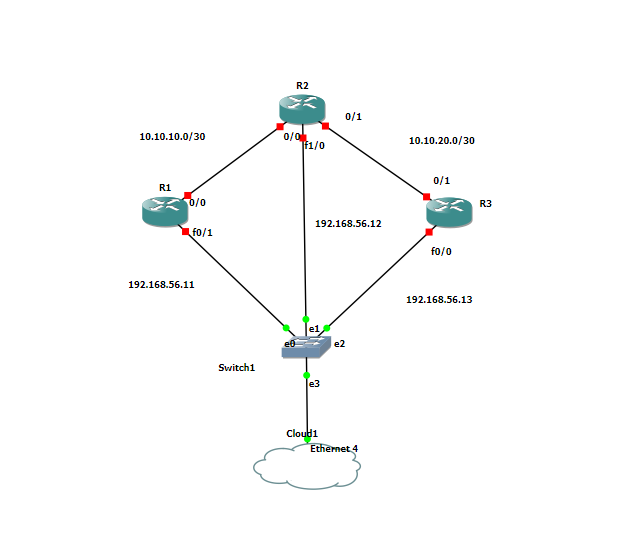
\includegraphics[width=0.85\textwidth]{imagenes/image27.png}
\caption{Topología de red empleada en GNS3 para la monitorización de los routers Cisco.}
\label{fig:topologia_gns3}
\end{figure}

Los elementos principales de la topología son los siguientes:

\begin{itemize}
    \item Router R1: primer dispositivo monitorizado, conectado a R2 mediante un enlace punto a punto y al switch mediante 
	la red 192.168.56.0/24.
    \item Router R2: nodo central de la topología, conectado tanto con R1 como con R3 a través de enlaces dedicados /30. Además, 
	posee acceso directo al switch a través de su interfaz f1/0.
    \item Router R3: router final de la topología, enlazado a R2 mediante un enlace punto a punto y conectado al switch mediante 
	la red LAN 192.168.56.0/24.
    \item Switch1: actúa como punto de conexión común entre los tres routers y el nodo Cloud.
    \item Cloud1: vinculado al adaptador Host-Only de VirtualBox, permite la comunicación entre GNS3 y la máquina virtual 
	Ubuntu que ejecuta el backend FastAPI.
\end{itemize}

\subsection*{Direccionamiento IP de la topología}

El direccionamiento configurado se divide en dos bloques principales: enlaces dedicados /30 entre routers y la red LAN 192.168.56.0/24 destinada a la comunicación con el servidor.

\subsubsection*{Enlaces punto a punto entre routers}

Los enlaces entre routers se configuñraron con subredes /30, adecuadas para enlaces dedicados:

\begin{itemize}
    \item R1–R2: red \texttt{10.10.10.0/30}
    \begin{itemize}
        \item R1 \texttt{f0/0}: \texttt{10.10.10.1}
        \item R2 \texttt{f0/0}: \texttt{10.10.10.2}
    \end{itemize}

    \item R2–R3: red \texttt{10.10.20.0/30}
    \begin{itemize}
        \item R2 \texttt{f0/1}: \texttt{10.10.20.1}
        \item R3 \texttt{f0/1}: \texttt{10.10.20.2}
    \end{itemize}
\end{itemize}

\subsubsection*{Red local compartida 192.168.56.0/24}

Los tres routers y la máquina virtual Ubuntu comparten la subred:

\[
192.168.56.0/24
\]

con la siguiente asignación:

\begin{itemize}
    \item R1 \texttt{f0/1}: \texttt{192.168.56.11}
    \item R2 \texttt{f1/0}: \texttt{192.168.56.12}
    \item R3 \texttt{f0/0}: \texttt{192.168.56.13}
    \item Servidor Ubuntu (interfaz \texttt{enp0s8}): \texttt{192.168.56.10}
    \item Adaptador Host-Only de VirtualBox: \texttt{192.168.56.1}
\end{itemize}

\subsection*{Conexión entre GNS3 y la máquina virtual}

La comunicación entre el entorno de simulación y el servidor se consigue mediante el nodo \textit{Cloud1}, configurado para utilizar el adaptador \textit{VirtualBox Host-Only} (Ethernet4). El flujo de comunicación es el siguiente:

\begin{enumerate}
    \item El servidor FastAPI envía solicitudes SSH hacia la red \texttt{192.168.56.0/24}.
    \item Estas solicitudes son reenviadas por el adaptador Host-Only al nodo \textit{Cloud1}.
    \item El nodo \textit{Cloud1} introduce los paquetes en el switch virtual.
    \item El switch reenvía el tráfico al router correspondiente según su dirección IP.
\end{enumerate}

De esta forma, la máquina virtual puede acceder a cualquiera de los routers simulados, ejecutar comandos IOS y recibir sus resultados.

\section{Diseño de la comunicación y flujo de datos}

Para garantizar una interacción fluida, segura y en tiempo real, se ha diseñado un flujo estructurado basado en el modelo cliente-servidor, en el que el frontend y el backend intercambian información mediante peticiones HTTP, mientras que la comunicación con los routers Cisco se realiza a través del protoclo SSH. En este apartado se describe con detalle el flujo completo de datos, desde la interacción del usuario hasta la ejecución de comandos en los routers y la posterior visualización de los resultados en la interfaz web.

\subsection*{Visión general del flujo de comunicación}

El sistema sigue un flujo secuencial bien definido:

\begin{enumerate}
    \item El usuario interactúa con la aplicación web desarrollada en Vue.js.
    \item El frontend envía peticiones HTTP al backend mediante Axios.
    \item El backend (FastAPI) valida la autenticación mediante tokens JWT.
    \item Si la petición requiere información del router, el backend establece una sesión SSH mediante la librería Paramiko.
    \item Se ejecutan los comandos IOS necesarios en el router.
    \item El backend procesa y estructura la salida obtenida en formato JSON.
    \item Los datos se envían de vuelta al frontend para su presentación.
\end{enumerate}

\subsection*{Flujo detallado de una petición típica}

A modo de ejemplo, se describe el proceso completo de consulta del estado de las interfaces de un router:

\begin{enumerate}
    \item El usuario selecciona un router desde la interfaz web.
    \item Vue.js envía una petición \texttt{GET} al endpoint \\ \texttt{/interfaces/\{router\_id\}}.
    \item Axios adjunta automáticamente el token JWT en la cabecera \texttt{Authorization}.
    \item FastAPI verifica la validez del token y autentica al usuario.
    \item El backend consulta su base de datos para obtener la dirección IP del router solicitado.
    \item Se inicia una sesión SSH con el router utilizando Paramiko.
    \item FastAPI ejecuta comandos IOS como:
    \begin{itemize}
        \item \texttt{show ip interface brief}
        \item \texttt{show interfaces}
        \item \texttt{show interfaces counters errors}
    \end{itemize}
    \item La salida se procesa para extraer únicamente la información relevante.
    \item El backend genera un objeto JSON estructurado con los datos del router.
    \item Vue.js recibe los datos y actualiza dinámicamente la vista mediante componentes reactivos.
\end{enumerate}

Este flujo se repite cada vez que el sistema necesita actualizar la información mostrada al ususario.

La Figura~\ref{fig:flujo_comunicacion} representa de forma gráfica el proceso descrito anteriormente, destacando la interacción entre los distintos componentes del sistema: usario, frontend, backend y routers Cisco.

\begin{figure}[H]
\centering
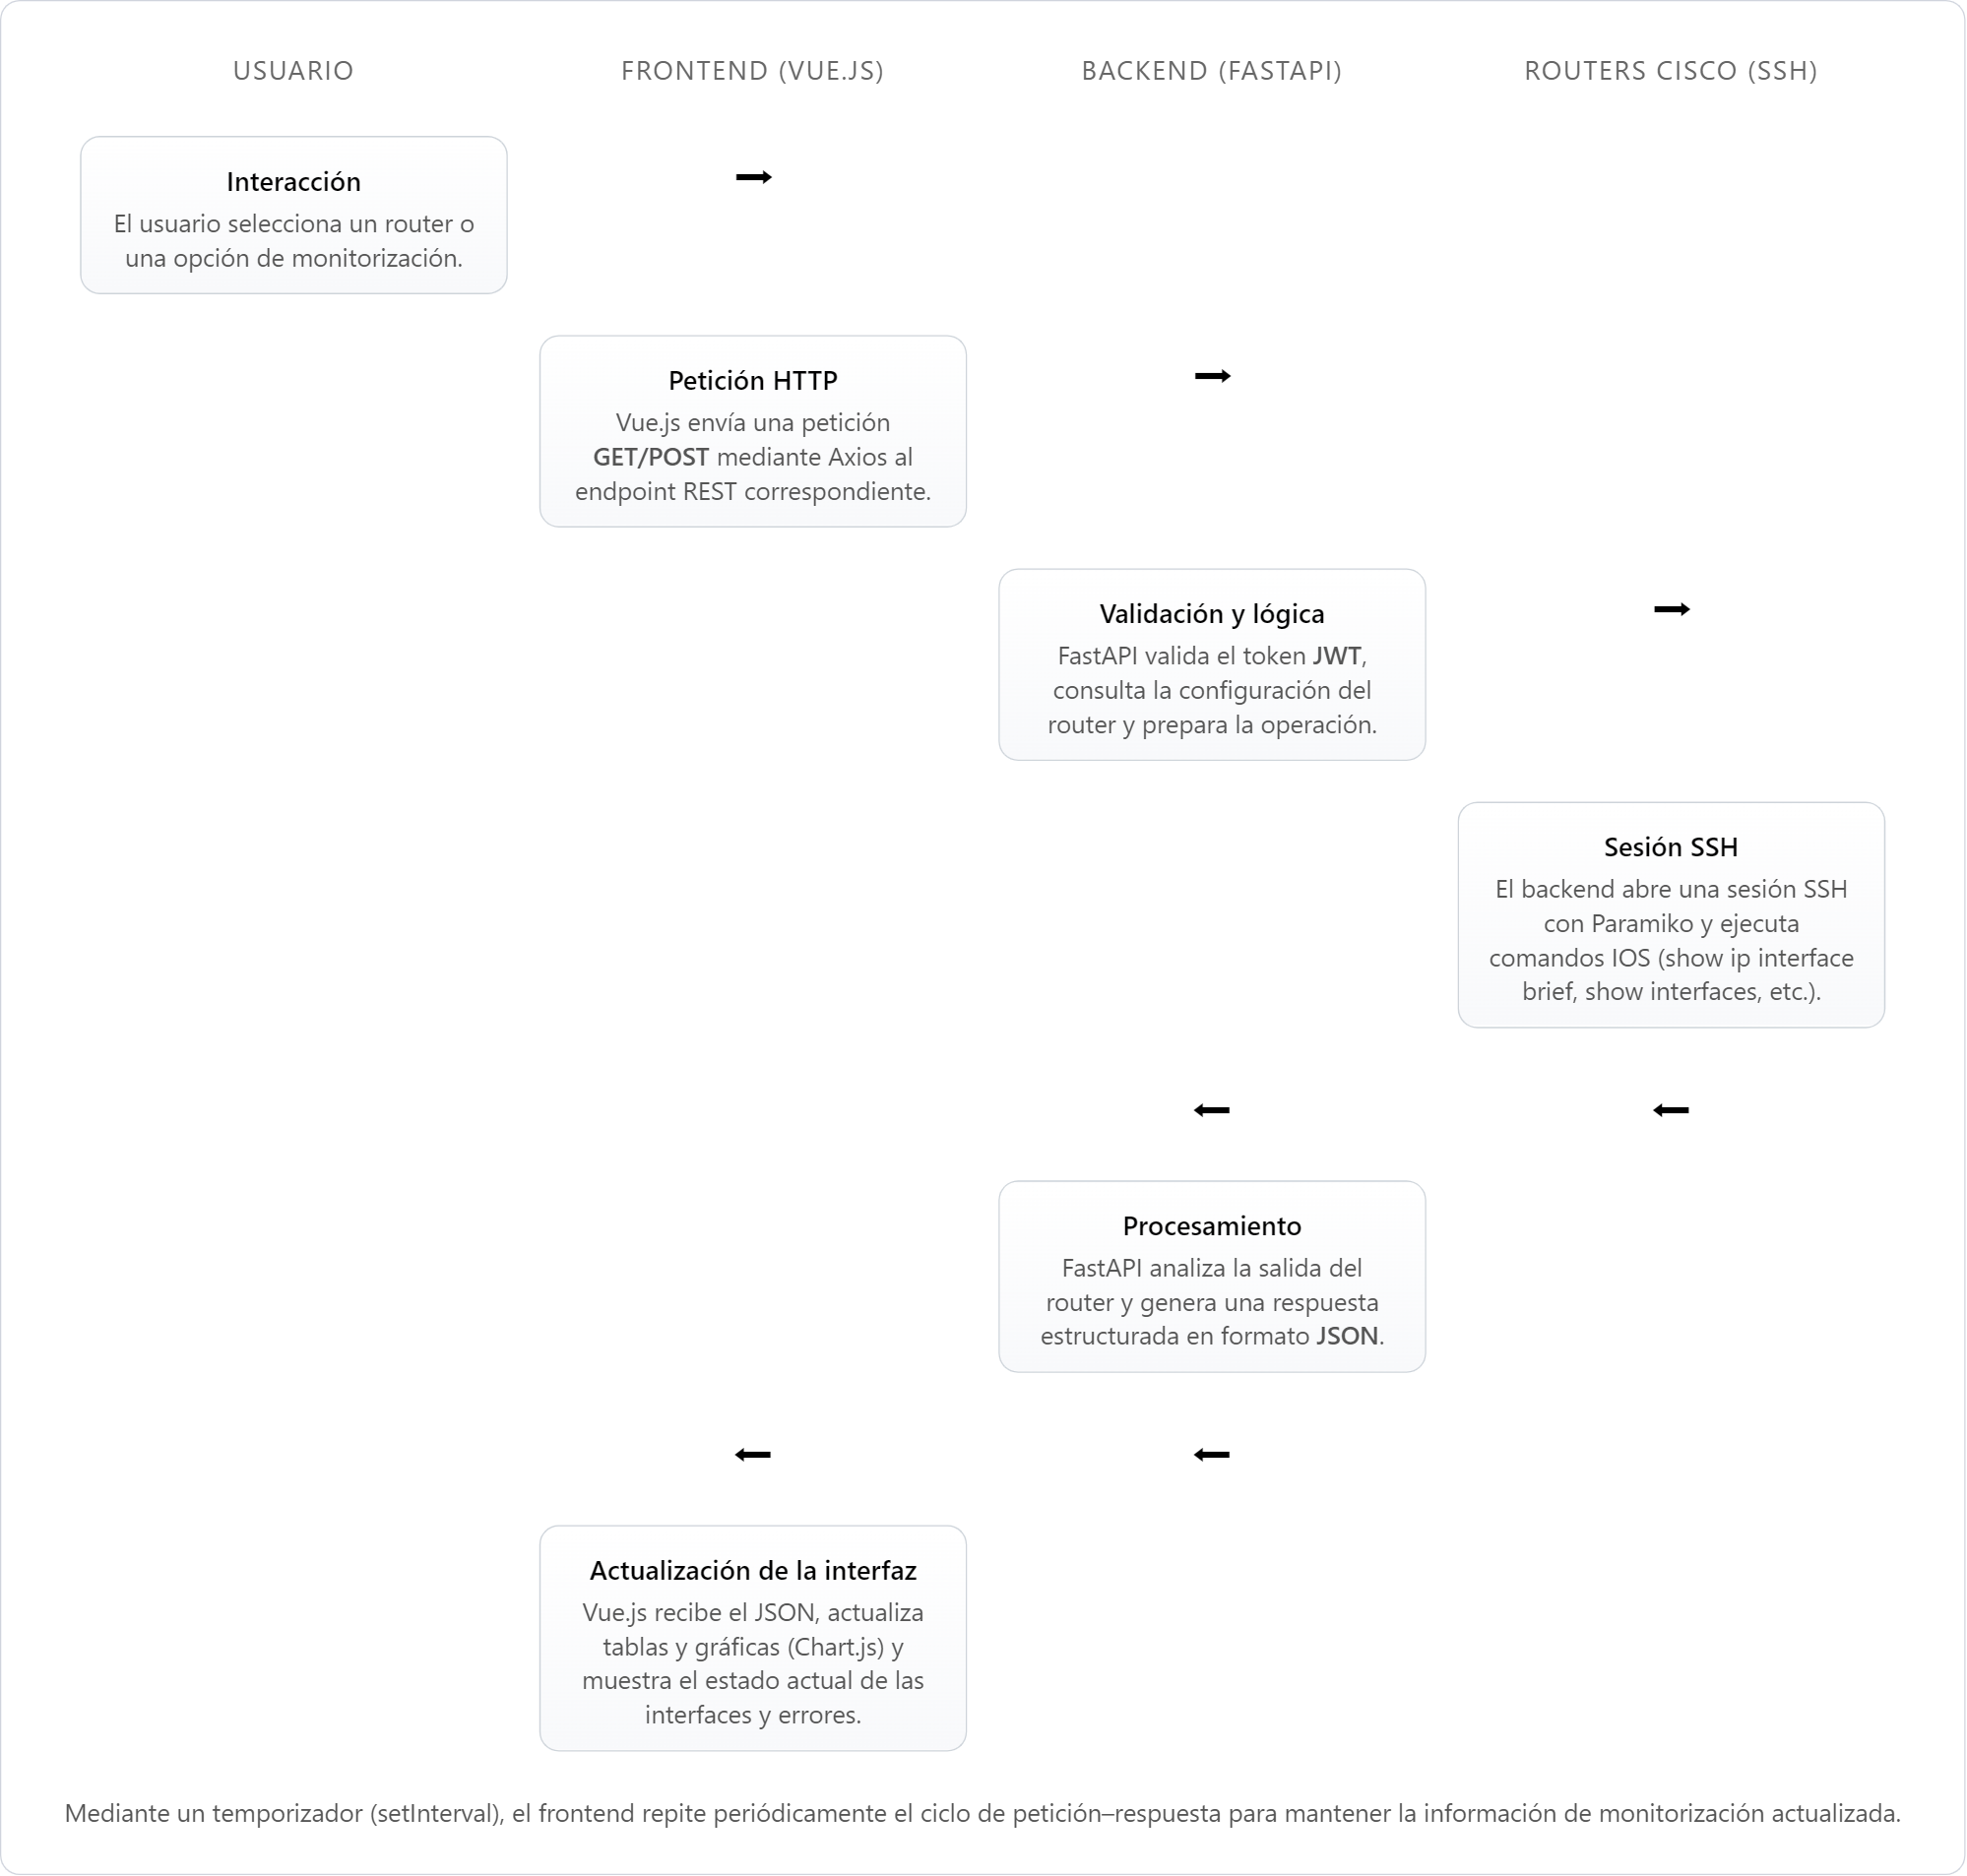
\includegraphics[width=0.85\textwidth]{canva/flujo_comunicacion.png}
\caption{Diagrama del flujo de comunicación entre el usuario, el backend y los routers Cisco.}
\label{fig:flujo_comunicacion}
\end{figure}

\subsection*{Intercambio de datos en formato JSON}

El backend devuelve toda la información al frontend mediante resupuestas en formato JSON, lo que facilita su interpretación y representación gráfica. Un ejemplo simplificado de la respuesta generada por el endpoint \texttt{/interfaces/\{router\_id\}} es el siguiente:

\begin{verbatim}
{
  "interfaces": [
    {
      "name": "FastEthernet0/0",
      "ip": "192.168.56.12",
      "status": "up",
      "protocol": "up"
    },
    {
      "name": "FastEthernet0/1",
      "ip": "unassigned",
      "status": "down",
      "protocol": "down"
    }
  ]
}
\end{verbatim}

\subsection*{Actualización periódica de los datos}

Para garantizar la monitorización en tiempo real, el frontend realiza solicitudes periódicas al backend utilizando la función \texttt{setInterval()}. Asegurando que el usuario visualice constantemente información actualizada. Durante cada ciclo de actualización:

\begin{enumerate}
    \item Se destruyen las gráficas anteriores para evitar errores en Chart.js.
    \item Se solicitan los datos actualizados del router.
    \item La interfaz vuelve a generarse con los nuevos valores.
\end{enumerate}